
%
%%%%%%%%%%%%%%%%%%%%%%%%%%%%%%%%%%%%%%%%%%%%%%%%%%%%%%%%%%%%%%%%%%%%%%%%%%%%%%%%%
%\subsection{Технические средства}  %% Список не удалять!!!
%\begin{itemize}
%%
%%%
%%%\item   Диагностический сканер SDconnect   с программным обеспечением Xentry Diagnostics v19.11.3.1
%%
%\item   Линейка масштабная магнитная с цветографической шкалой, 100мм
%%
%%%\item   Рулетка измерительная металлическая, 5м
%%%\item  Универсальный стенд для измерения углов установки колес Hunter Engineering %ProAlign с программным инструментом регулировки схождения колес без блокировки руля %автомобиля WinToe
%\item 	Цифровой фотоаппарат Canon 760D s/n 143032001327 с объективом Canon EF-S 18-135, тип используемой памяти: Transcend,  32Gb
%%
%%\item  Специализированное программное обеспечение для расчёта стоимости  восстановительного ремонта, содержащее нормативы трудоёмкости работ, регламентируемые изготовителями транспортного средства     AudaPadWeb, лицензионное соглашение № AS/\- APW-658  RU-P-409-
%\item  Специализированное программное обеспечение для расчёта стоимости  восстановительного ремонта, содержащее нормативы трудоёмкости работ, регламентируемые изготовителями транспортного средства  SilverDAT myClaim,
%лицензионный договор № 1422 от 05.02.2021 на право использования программы для ЭВМ от  DAT IP-Management und Vertriebs GmbH.
%
%%
%\item  Программа обработки фото-видео изображений ImageJ, разработчик  Wayne Rasband (wa-yne@codon.nih.gov),
%свободная лицензия GPL
%%
%\item  ПЭВМ под управлением операционной системы Windows 10 с установленным набором макрорасширений LaTeX системы компьютерной вёрстки TeX, cвободная лицензия LaTeX Project Public License (LPPL)
%%	
%\end{itemize}
%%%%%%%%%%%%%%%%%%%%%%%%%%%%%%%%%%%%%%%%%%%%%%%%%%%%%%%%%%%%%%%%%%%%%%%%%%%%%%%%%%%%%%%%%%%%%%%%%%%%%%

\subsection{Методы исследования}
\begin{itemize}
\item  Органолептический метод – исследование и оценка качества объектов с помощью органов чувств
\item 	Прямой измерительный метод – путем измерения размеров деталей специальными измерительными приборами
\item Расчётный метод (косвенный измерительный метод) – путём расчётов различных параметров на основе результатов измерений и других данных
\item Экспертный метод (метод экспертной оценки) — совокупности операций по выбору комплекса или единичных характеристик объекта, определению их действительных значений и оценкой экспертом соответствия их установленным требованиям и/или технической информации
%\item Метод натурной реконструкции??
\end{itemize}


%\subsection{Исходные данные}
%
%\begin{enumerate}
%	
%	\item Автомобиль \тс \, VIN \vin \, в повреждённом состоянии.
%	\item Цифровая копия видеозаписи \enquote{улица парковка 3\_23\_06\_2020 06.43.00.mp4}, формата  MPEG-4,  размером 33.4 MiB, длительностью 1 min 59 s, 12.275 FPS.
%	\item Светокопия постановления № 18810223177772659936 от 23.06.2020г. по делу об административном правонарушении, 2 лист.
%	\item Светокопия  решения к делу № 12-541/2020 УИД 23RS0041-01-2020-011330-91, 4 листа.
%%	
%%	
%\end{enumerate}

%%           
%\subsection{Обстоятельства дела}
%%
%%\begin{itemize}
%	%
%\item 
...............................................................
	

	%
%\end{itemize} 
%
%
\section{Исследование}
%

\subsection{Исследование предоставленных на экспертизу документов}
%

В соответствии с открытыми каталогами запасных частей  автомобиль с VIN \vin \ имеет следующие идентификационные характеристики:

\begin{figure}[H]
	\centering
	\includegraphics[width=0.7\linewidth]{example-image}
	\caption{Информация расшифровки VIN \vin \ по данным кталога \url{https://partsouq.com/}}
	\label{vin}
\end{figure}
%
17.07.2020 г. ООО «Элерон», г. Ростов-на-Дону (Продавец), ООО «Интерлизинг», г. Санкт Петербург (Покупатель) и ИП Мирзаева А.М., Краснодарский край, Белореченский район (Лизингополучатель) заключили договор купли-продажи № КП-23-2674/20 от 17.07.2020 г. Предметом данного договора стал новый автомобиль марка, модель, год выпуска, VIN которого соответствуют записям в свидетельстве о регистрации ТС 9927 № 411797. Цена договора 6 850 000 руб.

Согласно договору купли-продажи № КП-23-2674/20 от 17.07.2020 исследуемый автомобиль  соответствует  автомобилю со следующими характеристиками:\\

\begin{figure}[H]
	\centering
	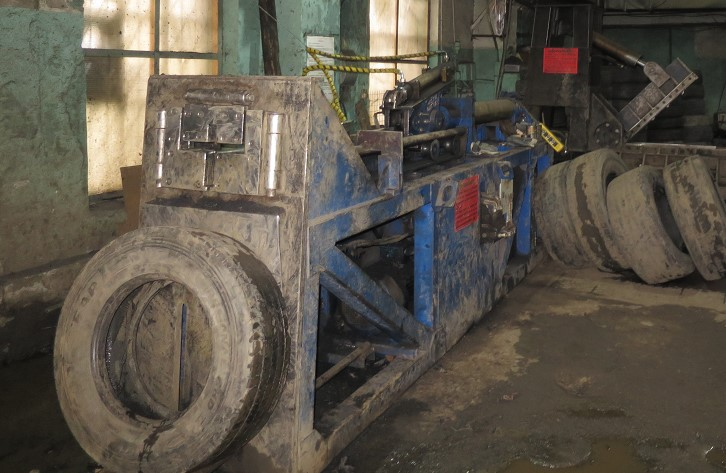
\includegraphics[width=0.99\linewidth]{1}
	\caption{Характеристики автомобиля.  Приложение №1 к договору купли-продажи № КП-23-2674/20 от 17.07.2020 г.}
	\label{vin}
\end{figure}

Полный перечень комплектации ТС содержится в договоре купли-продажи № КП-23-2674/20 от 17.07.2020.\\
Согласно  записям  выписки из электронной сервисной книжки автомобиля AUDI Q8, VIN  WAUZZZF15LD024287 поставка автомобиля приобретателю произведена   28.07.2020 г. Согласно условиям договора, автомобиль находится на расширенной гарантии до 27.07.2024 г. или достижения  пробег 120 000 км, при условии, что в первые 24 месяца пробег автомобиля не превысит 120 000 км. Гарантия на лако-красочное покрытие автомобиля составляет 36 месяцев с момента передачи автомобиля покупателю без ограничения пробега.\\[3mm]

В результате исследования предоставленных материалов, анализа актов выполненных работ  специалистами установлена  история ремонтов и сервисного обслуживания  транспортного средства VIN \vin. Результаты исследования представлены ниже в таблице \ref{tab:hist}.
%%%%%%%%%%%%%%%%%%%%%%%%%%%%%%%%%%%%%
% История автомобиля
%%%%%%%%%%%%%%%%%%%%%%%%%%%%%%%%%%%%%
%{\small 
%	\begin{longtable}{|p{16mm}|p{12mm}|p{29mm}|G{50mm}|G{41mm}|}
%		\caption[]{\footnotesize {\textbf{История ремонта и сервисного обслуживания по дате и пробегу}}} \label{tab:hist}\\
%		\hline
%		%\rowcolor[HTML]{C0C0C0} 
%		% Заголовки столбцов
%		\textbf{Дата} &\textbf{Пробег, км} &\textbf{№\,Заказ-наряда, накладной}& \textbf{Вид работы}& \textbf{Примечание} \\ \hline \endhead % повторение заголовка 
%		% Строки
%%		22.22.2019 &33\,000  & № 480279303-1 от 03.09.2019& Панель задка  & Замена, окраска \\ \hline
%%		%\rowcolor[HTML]{EFEFEF} 
%%		\Rownum & &n & Боковина задняя левая   & Замена, окраска \\ \hline
%		
%		\ист{arg1}{arg2}{arg3}{arg4}{arg5}
%		\ист{arg1}{arg2}{arg3}{arg4}{arg5}
%		\ист{arg1}{arg2}{arg3}{arg4}{arg5}
%		
%		
%		%%% ..............& 
%		% Обнуляем счетчик строк для следующей таблицы
%\end{longtable}}
%\setcounter{rownum}{0} %сброс счетчика строк в таблице


{\footnotesize \
	\begin{longtable}[h]{m{5mm}|m{14mm}|m{13mm}|m{35mm}|m{50mm}|m{18mm}}
	\caption[]{\footnotesize {\textbf{История ремонта и сервисного обслуживания по дате и пробегу}}} \label{tab:hist} \\ \hline
		\textit{\textbf{n/n}} 
		&\textit{\textbf{Дата}} 
		&\textit{\textbf{Пробег, км}}
		&\textit{\textbf{Документ}} 
		&\textit{\textbf{Содержание}} 
		&\textit{\textbf{Примечание}}\\ \hline \endhead
		

		\Rownum &27.05.2020& -- & Информация VIN & Дата изготовления автомобиля &Данные сайта  partsouq.com\\
		\hline
		\Rownum &17.07.2020& -- & Договор купли продажи автомобиля №КП-23-2674/20 от 17.07.2020г..& Покупка нового  автомобиля ООО «Интерлизинг» для ИП Мирзаева А.М.& -- \\
		\hline
		
		\Rownum &27.07.2020& 0 & 420198409-1 & Предпродажная подготовка & "Элерон" \\
		\hline
			\Rownum &28.07.2020& 0 & Выполнение  условий договора & Поставка ТС приобретателю & "Элерон" \\
		\hline
		
		
			\Rownum &20.11.2020& 14 258 & 420201825-1 & Замена масла, сажевого фильтра & "Элерон" \\
		\hline
		
		
		\Rownum &13.06.2021& 19 379& Акт выполненных работ №430092116-/ 430092116-1 от 13.09.2021 г.  & Причина обращения со слов клиента: диагностика.
		Выполненные работы: ведомый поиск неисправностей; диагностика ходовой части; геометрия передней и задней частей автомобиля проверить.
		Рекомендации сервиса: выполнить проверку развал-схождения; выполнить чистку дроссельных заслонок; произвести антибактериальную обработку климата; заменить лобовое стекло; приклеить плёнку на правой передней арке колеса и решетке радиатора & ООО «Формула-АЦК2»\\
		\hline
		\Rownum 	&13.09.2021& 29 203& Акт выполненных работ №430096159-1 от 13.09.2021 г. & Причина обращения со слов клиента: ошибка по замку задней левой двери.
		Выполненные работы: ведомый поиск неисправностей; обновление ПО блока управления коробки передач.
		Рекомендации сервиса: при включении задней скорости периодически не работает ра заднего вида - в момент нахождения автомобиля в сервисе неисправность не проявляется; & ООО «Формула-АЦК2». Гарантийный ремонт\\
		\hline
		\Rownum 	&19.09.2021& 29 203& Акт выполненных работ №430096060-/ 430096060-1 от 19.09.2021 г.  & Причина обращения со слов клиента: ТО-2.
		Выполненные работы: замена масла моторного НХ8 Syn 5W-30, масляного фильтра 059198405, топливного фильтра 4М0127434Н, воздушного фильтра 4М0133843С, салонного фильтра 
		PF2357, тормозных колодок 4M0698151K, кабеля предупредительных сигналов 4M0615121AB.
		Рекомендации сервиса: выполнить проверку развал-схождения; выполнить чистку дроссельных заслонок; произвести антибактериальную обработку климата; заменить лобовое стекло; приклеить плёнку на правой передней арке колеса и решетке радиатора& ООО «Формула-АЦК2».  ТО-2 \\
		\hline
		\Rownum 	&04.10.2021& 31 040& Акт выполненных работ №430097287-/ 430097287-1 от 04.10.2021 г.  & Причина обращения со слов клиента: замена щёток стеклоочистителей.
		Выполненные работы: замена щёток стеклоочистителя 4М8955425Е и 4М899800; проверка наружных световых приборов, проверка звукового сигнала; проверка уровня тормозной жидкости, регулировка форсунок омывателя ветрового стекла; проверка давления в шинах, диагностика ходовой части.
		Рекомендации сервиса: выполнить проверку развал-схождения; выполнить чистку дроссельных заслонок; произвести антибактериальную обработку климата; заменить лобовое стекло; приклеить плёнку на правой передней арке колеса и решетке радиатора& ООО «Формула-АЦК2»\\
		\hline
		\Rownum 	&28.05.2022 & 42 616 & Акт выполненных работ №430105673-1 от 28.05.2022 г.  & Причина обращения со слов клиента: высветилась неисправность тормозной системы, пропали тормоза. Автомобиль на эвакуатора.
		Выполненные работы: ведомый поиск неисправностей; замена прокладки 059129717S, уплотнительного кольца 059129796J, вакуумной трубки 059131057Q, кронштейна 059131338M, вакуумного шланга 059131375АP, вакуумной трубки 059131377АD, прокладки 059131599R, вакуумной трубки 059131995E, прокладки 059145774A, электромагнитного клапана 059906283C, пневматического клапана 059906627P, шланга ОЖ с быстрораз 4M0122449AC, воздушного фильтра 4M0133837S, гидроблока ABS 4M6614517BBBEF; переоборудование впуска вакуумного насоса на впуск со шлангом для чистого воздуха
		Рекомендации сервиса: нет &ООО «Формула-АЦК2». Гарантийный ремонт\\	\hline
		\Rownum &28.05.2022& 42 616 & Акт выполненных работ № 430107020-/430107020-1 от 28.05.2022 г. & Причина обращения со слов клиента: ТО, переклеить плёнку переднего правого стекла, заменить масло и фильтр АКП (масло и фильтр свои оригинал).
		Выполненные работы: замена масла 
		LGENSPECVN5W3O и фильтра АКПП оЕ671 3, замена салонного фильтра PF2357, замена плёнки AIR 90CL HPR (30,5*1,525) 46,5м2 Llumar/ с логотипом на лайнере, проверка наружных световых приборов, проверка звукового сигнала; проверка уровня масла в двигателе,  проверка уровня тормозной жидкости, регулировка форсунок омывателя ветрового стекла; проверка давления в шинах, диагностика ходовой части
		Рекомендации сервиса: нет&  ООО «Формула-АЦК2».   ТО \\
		\hline
		\Rownum 	&29.08.2022& 53 677& Акт выполненных работ № 430107437-1 от 29.08.2022 г. & Причина обращения со слов клиента: -
		Выполненные работы: ведомый поиск неисправностей, замена датчика числе оборотов ABS 01500000
		Рекомендации сервиса: нет& ООО «Формула-АЦК2». Гарантийный ремонт \\
		\hline
		\Rownum 	&29.08.2022& 53 677& Акт выполненных работ №430110328-1 от 29.08.2022 г. & Причина обращения со слов клиента: -
		Выполненные работы: ведомый поиск неисправностей, замена датчика перепада давления 26751939.
		Рекомендации сервиса: нет& ООО «Формула-АЦК2». Гарантийный ремонт \\
		\hline
		\Rownum 	& 30.09.2022 & 53 677& Акт выполненных работ №430111231-1 от 30.09.2022 г. & Причина обращения со слов клиента: -
		Выполненные работы: замена замков двери 58171950 и 58171950.
		Рекомендации сервиса: нет& ООО «Формула-АЦК2». Гарантийный ремонт  \\
		\hline
		
		
\end{longtable}}\setcounter{rownum}{0}

\noindent Анализ истории по характерным событиям и признакам позволяет выделить следующие значимые составляющие:
\begin{enumerate}
\item  
На момент настоящего исследования автомобиль находится на гарантии.
\item  
Сведения о нарушении графика ТО отсутствуют.
\item  
За весь период эксплуатации на автомобиле были выявлены неисправности системы замков  задних дверей  58171950 и 58171950, датчика перепада давления 26751939, датчика ABS переднего левого колеса, трубки с обратным клапаном 059131057Q,  гидроблока ABS 4M6614517BBBEF.
\item 
Причинами  всех неисправностей были признаны соответствующие производственные дефекты.  
\item 
Согласно предоставленных документов, все выявленные неисправности устранены по гарантии. 
\end{enumerate}


%%%%%%%%%%%%%%%%%%%%%%%%%%%%%%%%%%%%%%
% 
\subsection{Исследование транспортного средства}

Осмотр и диагностическое исследование  автомобиля AUDI Q8 г.р.з. А179ОК193, VIN WAUZZZF15LD024287  производились  по адресу: г. Краснодар, ул. Аэропортовская-4/а, на территории СТОА ООО «Формула-АЦК2» 03.04.2023 г. с 09 час. 15 мин. до 13 час 25 мин.  в условиях естественного и искусственного освещения с использованием производственных мощностей СТОА ООО «Формула-АЦК2» в присутствии инженера по гарантии СТОА ООО «Формула-АЦК2» Колесникова Александра Витальевича.\\
 05.04.2023 с 12:15 до 12:45 на территории  ООО «Формула-АЦК2» в присутствии Колесникова А.В. произведено дополнительное  диагностическое исследование ТС.

\subsubsection{Осмотр транспортного средства}

\дварядом{example-image}{Исследуемый автомобиль  \тс \, \vin}{example-image}{Исследуемый автомобиль  \тс \, \vin}
\дварядом{example-image}{}{VIN под ветровым стеклом}{example-image}{VIN на передней стойке}

Осмотр автомобиля производился  органолептическим методом. В процессе осмотра выполнялась фото и видео съемка объекта исследования цифровой фотокамерой.\\ 
Маркировочные обозначения, нанесенные на кузове ТС соответствуют записям регистрационных документов. Кузов автомобиля окрашен двухслойной эмалью черного цвета, боковые элементы, включая молдинги,  капот имеют дополнительное защитное покрытие прозрачной виниловой пленкой. Автомобиль оснащен легкосплавными пятнадцатиспицевыми колесами черного цвета Audi Sport и шинами  Continental SportConntact 6 размерностью  285х40 R22 Y XL. Тягово-сцепное устройство на автомобиле отсутствует. Внешне автомобиль соответствует товарным образцам автомобилей Audi Q8 2020 модельного года.    Показание одометра (пробег)  53 689 км.  Бортовое время и дата ТС  не соответствует текущему. Настройки даты и времени ТС в начале осмотра: 16:34  19.11.2022. \\
Боковые двери, дверь задка, капот, крышка лучка заливной горловины топливного бака автомобиля  не опечатаны. Автомобиль комплектный. Уровни технических жидкостей находятся в рекомендуемых диапазонах.  Тормозная жидкость прозрачная, светлая, без видимых загрязнений. Охлаждающая жидкость розового цвета, светлая, прозрачная, без видимых загрязнений. Моторное масло темного цвета, по масломерному щупу уровень несколько ниже среднего значения. Каплепадение \cite{техрегтамсоюз:тр}, следы  подтекания рабочих жидкостей  или запотевания отсутствуют. Внешнее состояние деталей, узлов и агрегатов подкапотного пространства соответствует исправному, наружные поверхности покрыты  слоем пыли. Загрязнение воздушного фильтра незначительное, замена воздушного фильтра не требуется. \\
  Автомобиль   имеет  наружные повреждения  элементов, по внешним признакам соответствующие эксплуатационным повреждениям (см. Приложение: фототаблица):\\
 - капот – имеет незначительную вмятину площадью 1/4 дм2  с повреждением лакокрасочного покрытия (ЛКП) на передней кромке. \\
 - бампер передний имеет следы остаточной деформации  в нижней передней левой части, выраженные в   растрескивании на пощади 1 дм2 слоя ЛКП под защитной пленкой; в правой нижней части  утрачено ЛКП на площади 1/4 дм2. \\
 - решетка левая бампера переднего  не имеет  штатной фиксации  в проеме бампера, вероятно  повреждение креплений решетки;\\
  - решетка правая бампера переднего  имеет глубокие  задиры наружной поверхности  на площади 0,2 дм2. \\
 - решетка радиатора незначительно деформирована с повреждением ЛКП в месте, смежном с местом повреждения капота;\\
 - крыло переднее левое имеет плавную несложную деформацию в виде вмятины  под надписью «S Line» на площади поверхности 1,3 дм2;\\ 
 - облицовка арки боковины задней правой имеет повреждение защитной пленки.\\
В процессе осмотра салона автомобиля повреждения облицовки дверей, панели крыши, боковых стоек, панели приборов не выявлено. Облицовка передних и задних сидений кожаная, повреждения облицовки сидений отсутствует. При осмотре коврика салона, справа и слева на полу задних пассажиров имеются загрязненные участки веществом темного цвета. \\ Облицовка рулевого колеса без повреждений. Механизмы электрической регулировки передних сидений и рулевого колеса исправны.\\
На включение зажигания автомобиль реагирует штатно. Органы управления исправны, неисправности мультимедийной системы отсутствуют.\\ Проверка сопряжения автомобиля с мобильным телефоном не проводилась.\\
При  осмотре установленного на подъемнике автомобиля выявлены повреждения облицовки пола наружной правой в виде разрыва длиной 10 см в передней части;\\  - деформация теплозащитного экрана тоннеля пола левого;\\ - деформация  поперечины пола в виде вмятины диаметром 3см в правой передней части;\\
 - деформации облицовки  правой  топливного бака в виде разрыва материала детали передней части;\\
- нарушение целостности защитного кожуха компрессора пневмоподвески\\ - деформация ребра редуктора заднего моста. \\
Отдельно необходимо отметить наличие признаков остаточной деформации панели задка в задней нижней  левой части.\\
 Перечисленные повреждения, по совокупности морфологических  признаков, получены в процессе эксплуатации автомобиля и не имеют  причинной, следственной связи с неисправностями, указанными в предоставленных актах выполненных работ. \\
 Отдельное внимание при осмотре автомобиля было уделено практической проверке работоспособности стеклоподъемников и доводчиков дверных замков. На момент настоящего исследования механизмы открывания/закрывания всех дверей исправны и демонстрируют штатную работу.\\
   Таким образом, при проведении  осмотра автомобиля были установлены незначительные механические повреждения наружных элементов  транспортного средства, деформация нижнего  ребра охлаждения корпуса редуктора заднего моста, незначительная деформация, не изменяющая базовую геометрию детали, нижней поперечной балки,   загрязнение салонного коврика в районе заднего ряда пассажирских сидений. Все имеющиеся повреждения  получены в процессе эксплуатации транспортного средства.\\
   05.04.2023 в 08:30  проведена проверка  по открытой информационной базе ГИБДД об участии ТС с VIN  WAUZZZF15LD024287 в зарегистрированных дорожно-транспортных происшествиях, \url{https://xn--90adear.xn--p1ai/check/auto#WAUZZZF15LD024287}. Установлено, что данный автомобиль был участником одного ДТП. 08.03.2021 в 01:45   совершен наезд на препятствие. 
   \begin{figure}[H]
   	\centering
   	\includegraphics[width=0.7\linewidth]{дтп1}
%   	\label{vin}
   \end{figure}
\begin{figure}[H]
	\centering
	\includegraphics[width=0.7\linewidth]{дтп2}
%	\label{vin}
\end{figure}
\begin{figure}[H]
	\centering
	\includegraphics[width=0.7\linewidth]{дтп3}
	\caption{Данные сайта \url{https://гибдд.рф}}
	\label{гибдд}
\end{figure}  
   
 По завершении наружного осмотра автомобиля, с целью разрешения вопросов настоящего исследования, проведена диагностика ТС VIN WAUZZZF15LD024287.  Диагностирование автомобиля проводилось программно-аппаратными средствами   официального дилера.  Согласно протокола диагностики от 03.04.2023  12:22 марка, тип, модельный год, модификация, буквенное обозначение двигателя, автоматически определенный VIN полностью соответствуют наружной маркировке автомобиля.\\
 Первоначально было сделано два протокола диагностики.  03.04.2023  12:22 и  03.04.2023  12:25.  По причине недостаточного уровня  напряжения АКБ автомобиля и неустойчивой связи WI-FI протокол от 03.04.2023 12:22 к рассмотрению не принимается.  Для корректного прочтения  кодов DTC автомобиль был подключен к зарядному модулю АКБ, случайно возникшие коды DTC стерты.  \\
 Следующий протокол диагностики от 03.04.2023  12:25 коды ошибок не содержит. Система самодиагностики  указывает на исправное состояние ТС.\\
 % Для дальнейшей проверки автомобиля были проведены дорожные испытания автомобиля. Перед началом движения  проведена проверка исправности световых приборов, возможности регулировки рулевого колеса, сиденья водителя и пассажира, свеклоподъемники боковых дверей, работа акустической системы, работа двигателя в режиме холостого хода. В статическом состоянии неисправности автомобиля не обнаружены. Ввиду отсутствия сим-карты в мультимедийной системе, исправность функционала, зависящего от наличия сим-карты не проверялась.  Движение автомобиля осуществлялось по территории сервисного центра без выезда на дороги общего пользования. Полотно дороги сухое, асфальтобетон, температура окружающего воздуха +18\град С.  Применялся  равномерный режим движения на постоянной скорости, переменный режим движения с чередованием ускорения и торможения, проезд неровностей в виде стандартных "лежачих полицейских" попеременно левыми и правыми колесами. Нефункциональные шумы, перебои в работе двигателя, подвески, коробки перемены передач и других системах автомобиля отсутствуют.   Торможение автомобиля штатное, многократное торможение происходит с одинаковым усилием, неисправности элементов тормозной системы отсутствуют. Работа АКПП штатная и соответствует работе исправного агрегата.\\   
% По результатам  дорожных испытаний специалисты приходят к заключению, что исследуемый автомобиль по состоянию на 03.04.2023 года находится в исправном техническом состоянии.\\
% После дорожных испытаний 
Затем  электронные системы автомобиля диагностировались еще дважды: 03.04.2023  12:49 и  05.04.2023 в 12:26. 
Согласно протокола диагностики от 03.04.2023  12:49  автомобиль технически исправен. \\
Согласно протокола диагностики от  05.04.2023  12:26  автомобиль технически исправен.\\

Таким образом, из совокупности результатов наружного осмотра,
% , 
% дорожных испытаний и 
 диагностического исследования электронных систем автомобиля, следует, что транспортное средство \тс \, VIN \vin \, по состоянию на 05.04.2023 года находится в исправном техническом состоянии. Передний бампер, капот, крыло переднее левое, решетка радиатора, решетка левая и правая бампера переднего, арка боковины задней правой, салонный коврик в районе заднего ряда сидений, ребро охлаждения редуктора заднего моста, детали защиты днища автомобиля имеют несущественные повреждения эксплуатационного характера, не оказывающие влияние на общее техническое состояние автомобиля. \\
% 05.04.2023 в 12:26  исследуемый автомобиль  продиагностирован  повторно. Так же, как и 03.04.2023 диагностика подтвердила отсутствие неисправностей автомобиля \тс VIN \vin.
  

%\subsubsection{Исследование наличия, характера и объёма технических повреждений}
%
%  Наличие, характер и объем технических повреждений транспортного средства \tc\, регистрационный знак \grz, исследованы в присутствии заинтересованных лиц,  зафиксированы в акте осмотра № \NomerDoc\,  (Приложение, <<Акт осмотра>> ),  и фотоматериалах (Приложение, <<Фототаблица>>) по принадлежности. Планируемые (предполагаемые) ремонтные воздействия для восстановления повреждённого  транспортного средства назначены экспертом-техником с учётом особенностей конструкции и рекомендаций изготовителя  транспортного средства, укрупненных показателей трудозатрат по кузовному ремонту и устранению перекосов проёмов и кузова легковых автомобилей иностранных производителей, приложение 3 к приложению к Положению Банка России от 19 сентября 2014 года № 432-П и приведены ниже в таблице \ref{tab:5}.

%Повреждения транспортного средства \тс \, регистрационный знак \грз\, определены экспертом по материалам гражданского дела \delonum\, и представлены ниже в таблице \ref{tab:6}

%\pagebreak
\begin{longtable}{G{3mm}|M{90mm}|G{60mm}}
	\caption[]{\footnotesize {Эксплуатационные дефекты, установленные при  осмотре ТС}} 
	\label{tab:6}\\ 
	\hline 
	\hline  \toprule 
	\bf  {\footnotesize  n/n}  &\bf {\small Наименование  детали с описанием повреждения} & \bf {\small Изображение} \\   \hline\hline  \toprule \endhead 
	%%%%___________________________________________________________________    
	\пов{Наименование детали - описание повреждений }{example-image}

\end{longtable}\setcounter{rownum}{0}

	
	%\subsubsection{Определение стоимости восстановительных расходов}

%		\subparagraph{} Протокол диагностики(длинный) 03.04.2023  12:49  
		
		%\subsection{Расчет рыночной стоимости ТС}


\par \indent Рыночная стоимость транспортного средства - наиболее вероятная стоимость, по которой транспортное средство может быть отчуждено на открытом рынке в условиях конкуренции, когда стороны сделки действуют разумно, располагая всей необходимой информацией, а на величине стоимости сделки не отражаются какие-либо чрезвычайные обстоятельства [4]. Рыночная стоимость транспортного средства  рассчитывается  для условий конкретных товарных рынков транспортных средств, соответствующих месту государственной регистрации транспортного средства потерпевшего.
\par Определение рыночной стоимости ТС может производится сравнительным и затратным подходом, а именно:  сравнительный анализ продаж (анализ информации о первичном и вторичном рынке АМТС в Российской Федерации);  затратный (с учетом износа АМТС).
\par В оценочной практике наиболее распространенным и предпочтительным является метод прямого сравнения продаж, в соответствии с которым стоимость объекта оценки определяется как средняя цена отобранных аналогов с последующими параметрическими и износными корректировками.   В цены аналогов не вносятся корректировки, если аналоги являются идентичными и равновозрастными объектами по отношению к объекту оценки. 
\par Общий алгоритм метода прямого сравнения продаж:
\begin{list}{-}{}
	\item сбор необходимой информации об объектах;
	\item  производится выборка цен на объекты;
\item  проверка полученной выборки на однородность путем расчета коэффициента вариации;
\item  при значении коэффициента вариации, не превышающем 20\%, определяется средняя цена, которая принимается за стоимость объекта [9]
\item  при превышении коэффициента вариации значения  20\%  выборка исследуется на наличие выбросов с использованием метода Граббса [9,10].
\end{list}
Рыночная стоимость ТС отражает его комплектацию, комплектность, фактическое техническое состояние, срок эксплуатации, пробег, условия, в которых оно эксплуатировалось, коньюктуру первичного и вторичного рынка ТС в регионе. В общем случае расчет рыночной стоимости производится по формуле:
\begin{equation}\label{eq:aa}
C_{\text{КТС}} = C_{cp}\left(1 \pm  \left( \frac{\text{П}_{\text{П}}}{100}\right) \pm\left( \frac{\text{П}_{\text{Э}}}{100}\right) \right) + C_{\text{ДОП}}, \text{руб}
\end{equation}

\noindent где: $C_\text{ср}$ -- средняя цена ТС, \text{руб};\\
$ \text{П}_\text{П}$ -- процентный показатель корректировки средней цены ТС по пробегу, \%;\\
$ C_\text{ДОП}$ -- дополнительное увеличение (уменьшение) стоимости в зависимости от его комплектации, наличия повреждений и акта их устранения, обновления составных частей, руб.\\
Корректировка средней цены ТС, исходя из его комплектности, опций комплектации, обновления составных частей, повреждений и акта их устранения определяется по формуле:
\begin{equation}\label{eq:b}
  C_\text{ДОП}=C_1\pm C_2\pm\left( C_P+C_M+C_\text{ЗЧ}\cdot\left( 1-\text{И}\right) +C_\text{УТС}\right), \text{руб}  
\end{equation} 
где:\\
$C_1$ --увеличение средней цены транспортного средства вследствие замены (обновления его частей в процессе эксплуатации, руб;\\
$ C_2$ -- изменение средней цены транспортного средства в зависимости опций его комплектации, руб;\\
 $ C_P $ -- стоимость ремонтных работ, руб;\\
 $C_M$--  стоимость материалов, руб;\\
 $C_\text{ЗЧ}  $ -- стоимость запасных частей, руб;\\
 $ C_\text{УТС} $ -- величина УТС, руб;\\
 $ \text{И} $ -- величина износа, \%;\\
 
Приоритетным способом определения рыночной стоимость TC
является метод сравнительного подхода, основанный на объективных справочных данных о ценах на подержанные автомобили  в регионе, где проводится оценка.
   
При определении стоимости транспортного средства сравнительным подходом экспертом были использованы  Интернет-источники сведений об аналогах (таблица \ref{tab:5}), содержащие краткое описание основных характеристик и технического состояния. 
 
\begin{longtable}{|p{5mm}|p{85mm}|c|p{60mm}|l|}
	\caption[]{\footnotesize {Описание ТС, идентичных оцениваему}} \label{tab:5}\\ 
	\hline
	%\rowcolor[HTML]{C0C0C0} 
	\rowcolor[HTML]{EFEFEF}
\bf	\text{n/n} &\bf  Описание аналога & \bf URL-адрес преложения  \\ \hline \endhead
		\toprule \centering
\Rownum  &\includegraphics[width=0.99\linewidth]{A_1} &{\noindent \scriptsize\ \url {https://auto.ru/krasnodar/cars/vaz/2107/1996-year/all}} \\ \hline 	\centering
%	\rowcolor[HTML]{EFEFEF} 
\Rownum  &\includegraphics[width=0.99\linewidth]{A_2} & {\noindent \scriptsize\ \url {https://auto.ru/krasnodar/cars/vaz/2107/1996-year/all}} \\ \hline 	\centering
\Rownum  &\includegraphics[width=0.99\linewidth]{A_3} &{\noindent \scriptsize\ \url {https://auto.ru/krasnodar/cars/vaz/2107/1996-year/all}} \\ \hline 	\centering
\Rownum  &\includegraphics[width=0.99\linewidth]{A_4} &{\noindent \scriptsize\ \url {https://auto.ru/krasnodar/cars/vaz/2107/1996-year/all}} \\ \hline 	\centering
\Rownum &\includegraphics[width=0.99\linewidth]{A_5} &{\noindent \scriptsize\ \url {https://auto.ru/krasnodar/cars/vaz/2107/1996-year/all}} \\ \hline 	\centering
\Rownum  &\includegraphics[width=0.99\linewidth]{A_6} &{\noindent \scriptsize\ \url {https://auto.ru/krasnodar/cars/vaz/2107/1996-year/all}}\\ \hline 	\centering
\Rownum  &\includegraphics[width=0.99\linewidth]{A_7} &{\noindent \scriptsize\ \url {https://krasnodar.drom.ru/data/2107/35131847}} \\ \hline 	\centering
%\Rownum  &\includegraphics[width=0.99\linewidth]{A_8} &{\noindent \scriptsize\ \url {https://https://krasnodar.drom.ru/lada/2107/34429407}} \\ \hline 	\centering \textbf{}
\Rownum &\includegraphics[width=0.99\linewidth]{A_9} &{\noindent \scriptsize\ 
\url {https://krasnodar.drom.ru/lada/2107/33456928}} \\ \hline
					
\end{longtable}
%}

%	1. Определяется \overline{X} – среднее значение цены в %промежуточной выборке по формуле:        
 %
%где n – объем выборки (количество элементов в выборке);
%X_i – цена\  i– го объекта-аналога в промежуточной выборке.
%
%	2. Проверяется полученная выборка на однородность путем расчета %коэффициента вариации. Степень однородности выборки оценивается по %коэффициенту вариации (VB ), измеряющему  рассеивание данных %относительно среднего значения:
%V_B=\frac{\sigma_1}{\overline{X}}100%,  
%где \sigma_1- среднеквадратическое (или стандартное) отклонение, %определяемое по формуле:
%\sigma_1=\sqrt{\frac{\sum_{i=1}^{n}{{(X}_i-\overline{X})}^2}{n-1}};
%D= \frac{\sum_{i=1}^{n}{{(X}_i-\overline{X})}^2}{n-1}, где D -%дисперсия выборки.
	%Для малой выборки принято считать, что если VB <15%, то %однородность выборки высокая; 15% <VB<<25%, однородность выборки %средняя,  25% < VB< 33% однородность выборки низкая [9].
	%4. .При значении коэффициента вариации, не превышающем 20%, %определяется средняя цена, которая принимается за стоимость объекта.
	%5.  При превышении коэффициента вариации значения  20%  выборка %исследуется на наличие выбросов с использованием метода Граббса.
	%Окончательно, рассчитанная средняя цена предложения корректируется %с учетом торга в зависимости  от активности рынка – чем выше %спрос/предложение, тем ниже корректировка на торг. Для данного ТС %наиболее вероятное значение корректировки – 10.9% (данные %аналитического агентства «Автостат» %%http://www.autostat.ru/news/20083/)











%%%%%%%%%% среднеквадратичное отклонение и дисперсия выборки
%где $ \sigma_1 $- среднеквадратическое (или стандартное) отклонение, определяемое по формуле:
%\begin{equation}\label{ab}
%\sigma_1=\sqrt{\frac{\sum\limits_{i=1}^{n}{{(X}_i-\overline{X})}^2}{n-1}}
%\end{equation}
%
%\begin{equation}\label{ac}
%D= \frac{\sum\limits_{i=1}^{n}{{(X}_i-\overline{X})}^2}{n-1}
%\end{equation},
%
%
%где $ D $ -дисперсия выборки.
%Для малой Для малой выборки принято считать, что если VB <15\%, то однородность выборки высокая; 15\% <$  V_B  $<<25\%, однородность выборки средняя,  25\% < VB< 33\% однородность выборки низкая 
%
%4. .При значении коэффициента вариации, не превышающем 20\%, определяется средняя цена, которая принимается за стоимость объекта.
%5.  При превышении коэффициента вариации значения  20\%  выборка исследуется на наличие выбросов с использованием метода Граббса.
%6.	Окончательно, рассчитанная средняя цена предложения корректируется с учетом торга в зависимости  от активности рынка – чем выше спрос/предложение, тем ниже корректировка на торг. Для данного ТС наиболее вероятное значение корректировки – 10.9\% (данные аналитического агентства «Автостат» http://www.autostat.ru/news/20083/)
%
%\par Рыночная стоимость ТС  учитывает его фактическое техническое состояние, условия, в которых оно эксплуатировалось.
% Ремонт кузовных составляющих транспортного средства является фактором, влияющим на уменьшение средней цены ТС. В соответствии с Методикой [1], Приложение 3.3 <<Процентный показатель корректирования средней цены КТС в зависимости от условий эксплуатации>>, Таблица 1, для автомобилей со сроком эксплуатации до 7 лет, при восстановлении трех и больше кузовных составных частей уменьшение рыночной стоимости составляет 10 \%. 

%\par При определении стоимости транспортного средства сравнительным подходом экспертом использованы  Интернет-источники сведений об аналогах (Таблица \ref{tab:5}), содержащие краткое описание основных характеристик и технического состояния. Поскольку при определении рыночной стоимости  эксперту-технику данные о техническом состоянии и условиях эксплуатации не заданы и объективно не могут быть  получены при осмотре ТС на момент исследования, то для расчета принимается следующее:
%\begin{list}{-}{}
%	\item техническое состояние ТС соответствует сроку эксплуатации;
%	\item тс не эксплуатировалось в режиме такси или специальных условий эксплуатации;
%	\item фактический пробег ТС на момент повреждения составлял 45 513 км;
%	\item  29.06.2018 г. ТС \тс \, участвовал в ДТП, в результате которого  автомобиль получил механические повреждения задней правой двери, заднего правого порога, заднего правого колеса,  подушки SRS справа.
%\end{list}

%Из открытых банков данных полиции следует, что автомобиль с VIN: \,  \вин\,  как минимум дважды становился участником ДТП.
%Первый раз 29.06.2018  06:40, извещение о ДТП № 030046913, в котором автомобиль получил повреждения задней правой двери, заднего правого порога, заднего правого колеса, подушки SRS справа, Рис. \ref{ris:images/d1} и второй раз 22.05.2019 06:50, извещение о ДТП № 030034947, в котором автомобиль получил повреждения деталей передней левой и задней частей кузова, Рис. \ref{ris:images/d2}.
%%
%\vspace{\baselineskip}
%%
%\begin{figure}[H]\centering
%	\parbox[t]{0.49\textwidth}
%	{\centering
%		\includegraphics[width=.49\textwidth]{images/d1}
%		\caption{\footnotesize {Повреждения в ДТП 29.06.2018 }}
%		\label{ris:images/d1}}
%	\hfil \hfil%раздвигаем боксы по горизонтали 
%	\parbox[t]{0.49\textwidth}
%	{\centering
%		\includegraphics[width=.49\textwidth]{images/d2}
%		\caption{\footnotesize {Повреждения в ДТП 22.05.2019}}
%		\label{ris:images/d2}}
%\end{figure}
%%
%\vspace{\baselineskip}
%
%{\noindent  \footnotesize \tikz \fill [red] (1,0.5) rectangle (0.1,0.1); --{\footnotesize  Вмятины, вырывы, заломы, перекосы, разрывы и другие повреждения с изменением геометрии элементов (деталей) кузова и эксплуатационных характеристик ТС.}\\
%	\tikz \fill [yellow] (1,0.5) rectangle (0.1,0.1); --  {\footnotesize Повреждения колёс (шин), элементов ходовой части, стекол, фар, указателей поворота, стоп-сигналов и других стеклянных элементов (в т.ч. зеркал), а также царапины, сколы, потертости лакокрасочного покрытия или пластиковых конструктивных деталей и другие повреждения без изменения геометрии элементов (деталей) кузова и эксплуатационных характеристик ТС.}\\[1mm]
%	
%\renewcommand\baselinestretch{1.2}\small\normalsize

%\par Вследствие вышеизложенного коэффициент $ C_\text{ДОП}$ принимается равным -10 \%, коэффициенты $ \text{П}_{\text{Э}} $ и $ \text{П}_{\text{П}} $ принимаем равными нулю.

Средняя цена  $C_\text{ср}$  определяется на базе  средней рыночной цены продажи совокупности идентичных ТС на дату оценки: 
\begin{equation}\label{C}
C_\text{ср} =   \frac{ \sum\limits_{i=1}^n{C_i}}{n}
\end{equation}
 $C_\text{ср} =(\sum\limits_{i=1}^n{C_i})/n= (35000+35000+38000+40000+35000+35000+40000+33000)/8 =36 375 $, руб.\\
\noindent где: $ C_i $ - цена предложения к продаже i-го ТС, \\
\indent i - количество предложений, i=8.
\par Поскольку используемая выборка состоит из цен предложений к продаже, то для приведения к средней рыночной цене покупки применяется коэффициент торга $ K_T $, значение которого согласно данных аналитического агентства «Автостат» http://www.autostat.ru/news/20083/, %рис. \ref{fig:avtostat} 
\, составляет 5 \%. Соответственно, средняя цена предложений должна быть скорректирована в соответствии с нижеприведенной формулой \ref{Cp}:
\begin{equation}\label{Cp}
C_\text{ср} =  \left( \sum\limits_{i=1}^n{C_i}\right)  \cdot K_T , \,\, \text{руб}
\end{equation}
%%%%%%%%%%%%%%%%%%%%%  График АВТОСТАТ (если нужно)
%\begin{figure}
%	\centering
%	\includegraphics[width=0.7\linewidth]{images/avtostat}
%	\caption{График аналитического агентства <<Автостат>> процента уторговывания по маркам автомобилей}
%	\label{fig:avtostat}
%\end{figure}
Тогда,\,\, рыночная стоимость $ C $ автомобиля \тс \, с учетом торга и факторов, влияющих на рыночную стоимость составляет: 
\begin{equation}\label{cp}
C = C_\text{ср} \cdot  K_T 
%-  C_\text{ДОП} 
= 36375 \cdot(100-5)
%)\cdot 0.9 
=  34556 \, \, \text{руб},
\end{equation} 
\noindent что с учетом округления составляет 35000  рублей.

\par Таким образом, рыночная стоимость ТС \тс, \, с учетом всех имеющихся сведений о состоянии ТС на момент повреждения \датадтп\,  составляет 35000 (Тридцать пять тысяч) рублей.

%\paragraph*{} Федеральным законом от 25.04.2002 года № 40-ФЗ «Об обязательном страховании гражданской ответственности владельцев транспортных средств» в редакции на момент заключения договоров страхования и страхового случая (далее – Закон об ОСАГО) установлено:
%(пункт 18 статьи 12) что размер подлежащих возмещению страховщиком убытков при причинении вреда имуществу потерпевшего определяется: \par а) в случае полной гибели имущества потерпевшего - в размере действительной стоимости имущества на день наступления страхового случая за вычетом стоимости годных остатков. Под полной гибелью понимаются случаи, при которых ремонт поврежденного имущества невозможен либо стоимость ремонта поврежденного имущества равна стоимости имущества на дату наступления страхового случая или превышает указанную стоимость.\par Настоящим исследованием установлено, что стоимость восстановительного ремонта ТС \тс \, превышает рыночную стоимость ТС на момент повреждения. Таким образом, при определении стоимости восстановительных расходов необходимо произвести расчет стоимости годных остатков ТС.
%\par  
%Положением Банка России от 19 сентября 2014 г. N 432-П "О единой методике определения размера расходов на восстановительный ремонт в отношении поврежденного транспортного средства <<Глава 5. Порядок расчета стоимости годных остатков в случае полной гибели транспортного средства>> установлен алгоритм расчета годных остатков ТС.




%	\subsection{Расчет рыночной стоимости ТС}


\par \indent Рыночная стоимость транспортного средства - наиболее вероятная стоимость, по которой транспортное средство может быть отчуждено на открытом рынке в условиях конкуренции, когда стороны сделки действуют разумно, располагая всей необходимой информацией, а на величине стоимости сделки не отражаются какие-либо чрезвычайные обстоятельства [4]. Рыночная стоимость транспортного средства  рассчитывается  для условий конкретных товарных рынков транспортных средств, соответствующих месту государственной регистрации транспортного средства потерпевшего.
\par Определение рыночной стоимости КТС, имеющего повреждения, которые предусматривают проведение восстановительного ремонта, затраты на его проведение рассчитывают на дату оценки [1, п.2.10].
\par Определение рыночной стоимости ТС может производится сравнительным и затратным подходом, а именно:  сравнительный анализ продаж (анализ информации о первичном и вторичном рынке АМТС в Российской Федерации);  затратный (с учетом износа АМТС).
%%%%%%%   ЗАТРАТНЫЙ ПОДХОД
\par Ввиду отсутствия на рынке аналогичных объектов сравнения для исследуемого автомобиля (новизна, начало продаж модели с 09.08.2019, эксклюзивность модели) определение рыночной стоимости исследуемого автомобиля производится затратным подходом.

\par Цена нового автомобиля  $  \text{Ц}_\text{нов} $ снижается после его продажи на величину $ K_\text{сниж} $, которая для автомобилей различных категорий может составлять до 30\%. По данным специализированных интернет-площадок, уменьшение стоимости автомобиля аналогичного сегмента рынка после продажи (утеря новизны) составляет 20\%. (\url{https://cenamashin.ru/cena/bmw/z4, automata.ru}).
%\noindent тогда
\begin{equation}\label{f:r}
\text{Ц}_\text{новприв} = \text{Ц}_\text{нов} \cdot (1-K_\text{сниж}/100)
\end{equation}

Цена нового АМТС   должна быть уменьшена с учетом эксплуатационного износа   по формуле:

\begin{equation}\label{f:n}
\text{Ц} = \text{Ц}_\text{новприв} \cdot (1-\text{И}_\text{э}/100)
\end{equation}

\noindent $ \text{Ц}_\text{новприв} = \text{Ц}_\text{нов}(1-K_\text{сниж}/100)= 5692000(1-20/100) = 4553600  $\\
\noindent $ \text{И}_\text{э} = 0,27\cdot3,697 = 1 \%  $\\
$ \text{Ц} = \text{Ц}_\text{новприв}(1-\text{И}_\text{э}/100) = 4553600(1-1/100) = 4508064 $ (Четыре миллиона пятьсот восемь тысяч шестьдесят четыре) рубля, что с учетом округления составляет 4500000 (Четыре миллиона пятьсот  тысяч) рублей.






%%%%%%%%%%%%%    СРАВНИТЕЛЬНЫЙ ПОДХОД
%\par В оценочной практике наиболее распространенным и предпочтительным является метод прямого сравнения продаж, в соответствии с которым стоимость объекта оценки определяется как средняя цена отобранных аналогов с последующими параметрическими и износными корректировками.   В цены аналогов не вносятся корректировки, если аналоги являются идентичными и равновозрастными объектами по отношению к объекту оценки. 
%\par Общий алгоритм метода прямого сравнения продаж:
%\begin{list}{-}{}
%	\item сбор необходимой информации об объектах;
%	\item  производится выборка цен на объекты;
%\item  проверка полученной выборки на однородность путем расчета коэффициента вариации;
%\item  при значении коэффициента вариации, не превышающем 20\%, определяется средняя цена, которая принимается за стоимость объекта [9]
%\item  при превышении коэффициента вариации значения  20\%  выборка исследуется на наличие выбросов с использованием метода Граббса [9,10].
%\end{list}
%Рыночная стоимость ТС отражает его комплектацию, комплектность, фактическое техническое состояние, срок эксплуатации, пробег, условия, в которых оно эксплуатировалось, коньюктуру первичного и вторичного рынка ТС в регионе. В общем случае расчет рыночной стоимости производится по формуле:
%\begin{equation}\label{eq:aa}
%C_{\text{КТС}} = C_{cp}\left(1 \pm  \left( \frac{\text{П}_{\text{П}}}{100}\right) \pm\left( \frac{\text{П}_{\text{Э}}}{100}\right) \right) + C_{\text{ДОП}}, \text{руб}
%\end{equation}
%
%\noindent где: $C_\text{ср}$ -- средняя цена ТС, \text{руб};\\
%$ \text{П}_\text{П}$ -- процентный показатель корректировки средней цены ТС по пробегу, \%;\\
%$ C_\text{ДОП}$ -- дополнительное увеличение (уменьшение) стоимости в зависимости от его комплектации, наличия повреждений и акта их устранения, обновления составных частей, руб.\\
%Корректировка средней цены ТС, исходя из его комплектности, опций комплектации, обновления составных частей, повреждений и акта их устранения определяется по формуле:
%\begin{equation}\label{eq:b}
%  C_\text{ДОП}=C_1\pm C_2\pm\left( C_P+C_M+C_\text{ЗЧ}\cdot\left( 1-\text{И}\right) +C_\text{УТС}\right), \text{руб}  
%\end{equation} 
%где:\\
%$C_1$ --увеличение средней цены транспортного средства вследствие замены (обновления его частей в процессе эксплуатации, руб;\\
%$ C_2$ -- изменение средней цены транспортного средства в зависимости опций его комплектации, руб;\\
% $ C_P $ -- стоимость ремонтных работ, руб;\\
% $C_M$--  стоимость материалов, руб;\\
% $C_\text{ЗЧ}  $ -- стоимость запасных частей, руб;\\
% $ C_\text{УТС} $ -- величина УТС, руб;\\
% $ \text{И} $ -- величина износа, \%;\\
% 
%Приоритетным способом определения рыночной стоимость TC
%является метод сравнительного подхода, основанный на объективных справочных данных о ценах на подержанные автомобили  в регионе, где проводится оценка.
%   
%При определении стоимости транспортного средства сравнительным подходом экспертом были использованы  Интернет-источники сведений об аналогах (таблица \ref{tab:5}), содержащие краткое описание основных характеристик и технического состояния. 
% 
%\begin{longtable}{|p{5mm}|p{85mm}|c|p{60mm}|l|}
%	\caption[]{\footnotesize {Описание ТС, идентичных оцениваему}} \label{tab:5}\\ 
%	\hline
%	%\rowcolor[HTML]{C0C0C0} 
%	\rowcolor[HTML]{EFEFEF}
%\bf	\text{n/n} &\bf  Описание аналога & \bf URL-адрес преложения  \\ \hline \endhead
%		\toprule \centering
%\Rownum  &\includegraphics[width=0.99\linewidth]{A_1} &{\noindent \scriptsize\ \url {https://auto.ru/krasnodar/cars/vaz/2107/1996-year/all}} \\ \hline 	\centering
%%	\rowcolor[HTML]{EFEFEF} 
%\Rownum  &\includegraphics[width=0.99\linewidth]{A_2} & {\noindent \scriptsize\ \url {https://auto.ru/krasnodar/cars/vaz/2107/1996-year/all}} \\ \hline 	\centering
%\Rownum  &\includegraphics[width=0.99\linewidth]{A_3} &{\noindent \scriptsize\ \url {https://auto.ru/krasnodar/cars/vaz/2107/1996-year/all}} \\ \hline 	\centering
%\Rownum  &\includegraphics[width=0.99\linewidth]{A_4} &{\noindent \scriptsize\ \url {https://auto.ru/krasnodar/cars/vaz/2107/1996-year/all}} \\ \hline 	\centering
%\Rownum &\includegraphics[width=0.99\linewidth]{A_5} &{\noindent \scriptsize\ \url {https://auto.ru/krasnodar/cars/vaz/2107/1996-year/all}} \\ \hline 	\centering
%\Rownum  &\includegraphics[width=0.99\linewidth]{A_6} &{\noindent \scriptsize\ \url {https://auto.ru/krasnodar/cars/vaz/2107/1996-year/all}}\\ \hline 	\centering
%\Rownum  &\includegraphics[width=0.99\linewidth]{A_7} &{\noindent \scriptsize\ \url {https://krasnodar.drom.ru/data/2107/35131847}} \\ \hline 	\centering
%%\Rownum  &\includegraphics[width=0.99\linewidth]{A_8} &{\noindent \scriptsize\ \url {https://https://krasnodar.drom.ru/lada/2107/34429407}} \\ \hline 	\centering \textbf{}
%\Rownum &\includegraphics[width=0.99\linewidth]{A_9} &{\noindent \scriptsize\ 
%\url {https://krasnodar.drom.ru/lada/2107/33456928}} \\ \hline
%					
%\end{longtable}
%%}
%
%%	1. Определяется \overline{X} – среднее значение цены в %промежуточной выборке по формуле:        
% %
%%где n – объем выборки (количество элементов в выборке);
%%X_i – цена\  i– го объекта-аналога в промежуточной выборке.
%%
%%	2. Проверяется полученная выборка на однородность путем расчета %коэффициента вариации. Степень однородности выборки оценивается по %коэффициенту вариации (VB ), измеряющему  рассеивание данных %относительно среднего значения:
%%V_B=\frac{\sigma_1}{\overline{X}}100%,  
%%где \sigma_1- среднеквадратическое (или стандартное) отклонение, %определяемое по формуле:
%%\sigma_1=\sqrt{\frac{\sum_{i=1}^{n}{{(X}_i-\overline{X})}^2}{n-1}};
%%D= \frac{\sum_{i=1}^{n}{{(X}_i-\overline{X})}^2}{n-1}, где D -%дисперсия выборки.
%	%Для малой выборки принято считать, что если VB <15%, то %однородность выборки высокая; 15% <VB<<25%, однородность выборки %средняя,  25% < VB< 33% однородность выборки низкая [9].
%	%4. .При значении коэффициента вариации, не превышающем 20%, %определяется средняя цена, которая принимается за стоимость объекта.
%	%5.  При превышении коэффициента вариации значения  20%  выборка %исследуется на наличие выбросов с использованием метода Граббса.
%	%Окончательно, рассчитанная средняя цена предложения корректируется %с учетом торга в зависимости  от активности рынка – чем выше %спрос/предложение, тем ниже корректировка на торг. Для данного ТС %наиболее вероятное значение корректировки – 10.9% (данные %аналитического агентства «Автостат» %%http://www.autostat.ru/news/20083/)
%
%
%
%
%
%
%
%
%
%
%
%%%%%%%%%%% среднеквадратичное отклонение и дисперсия выборки
%%где $ \sigma_1 $- среднеквадратическое (или стандартное) отклонение, определяемое по формуле:
%%\begin{equation}\label{ab}
%%\sigma_1=\sqrt{\frac{\sum\limits_{i=1}^{n}{{(X}_i-\overline{X})}^2}{n-1}}
%%\end{equation}
%%
%%\begin{equation}\label{ac}
%%D= \frac{\sum\limits_{i=1}^{n}{{(X}_i-\overline{X})}^2}{n-1}
%%\end{equation},
%%
%%
%%где $ D $ -дисперсия выборки.
%%Для малой Для малой выборки принято считать, что если VB <15\%, то однородность выборки высокая; 15\% <$  V_B  $<<25\%, однородность выборки средняя,  25\% < VB< 33\% однородность выборки низкая 
%%
%%4. .При значении коэффициента вариации, не превышающем 20\%, определяется средняя цена, которая принимается за стоимость объекта.
%%5.  При превышении коэффициента вариации значения  20\%  выборка исследуется на наличие выбросов с использованием метода Граббса.
%%6.	Окончательно, рассчитанная средняя цена предложения корректируется с учетом торга в зависимости  от активности рынка – чем выше спрос/предложение, тем ниже корректировка на торг. Для данного ТС наиболее вероятное значение корректировки – 10.9\% (данные аналитического агентства «Автостат» http://www.autostat.ru/news/20083/)
%%
%%\par Рыночная стоимость ТС  учитывает его фактическое техническое состояние, условия, в которых оно эксплуатировалось.
%% Ремонт кузовных составляющих транспортного средства является фактором, влияющим на уменьшение средней цены ТС. В соответствии с Методикой [1], Приложение 3.3 <<Процентный показатель корректирования средней цены КТС в зависимости от условий эксплуатации>>, Таблица 1, для автомобилей со сроком эксплуатации до 7 лет, при восстановлении трех и больше кузовных составных частей уменьшение рыночной стоимости составляет 10 \%. 
%
%%\par При определении стоимости транспортного средства сравнительным подходом экспертом использованы  Интернет-источники сведений об аналогах (Таблица \ref{tab:5}), содержащие краткое описание основных характеристик и технического состояния. Поскольку при определении рыночной стоимости  эксперту-технику данные о техническом состоянии и условиях эксплуатации не заданы и объективно не могут быть  получены при осмотре ТС на момент исследования, то для расчета принимается следующее:
%%\begin{list}{-}{}
%%	\item техническое состояние ТС соответствует сроку эксплуатации;
%%	\item тс не эксплуатировалось в режиме такси или специальных условий эксплуатации;
%%	\item фактический пробег ТС на момент повреждения составлял 45 513 км;
%%	\item  29.06.2018 г. ТС \тс \, участвовал в ДТП, в результате которого  автомобиль получил механические повреждения задней правой двери, заднего правого порога, заднего правого колеса,  подушки SRS справа.
%%\end{list}
%
%%Из открытых банков данных полиции следует, что автомобиль с VIN: \,  \вин\,  как минимум дважды становился участником ДТП.
%%Первый раз 29.06.2018  06:40, извещение о ДТП № 030046913, в котором автомобиль получил повреждения задней правой двери, заднего правого порога, заднего правого колеса, подушки SRS справа, Рис. \ref{ris:images/d1} и второй раз 22.05.2019 06:50, извещение о ДТП № 030034947, в котором автомобиль получил повреждения деталей передней левой и задней частей кузова, Рис. \ref{ris:images/d2}.
%%%
%%\vspace{\baselineskip}
%%%
%%\begin{figure}[H]\centering
%%	\parbox[t]{0.49\textwidth}
%%	{\centering
%%		\includegraphics[width=.49\textwidth]{images/d1}
%%		\caption{\footnotesize {Повреждения в ДТП 29.06.2018 }}
%%		\label{ris:images/d1}}
%%	\hfil \hfil%раздвигаем боксы по горизонтали 
%%	\parbox[t]{0.49\textwidth}
%%	{\centering
%%		\includegraphics[width=.49\textwidth]{images/d2}
%%		\caption{\footnotesize {Повреждения в ДТП 22.05.2019}}
%%		\label{ris:images/d2}}
%%\end{figure}
%%%
%%\vspace{\baselineskip}
%%
%%{\noindent  \footnotesize \tikz \fill [red] (1,0.5) rectangle (0.1,0.1); --{\footnotesize  Вмятины, вырывы, заломы, перекосы, разрывы и другие повреждения с изменением геометрии элементов (деталей) кузова и эксплуатационных характеристик ТС.}\\
%%	\tikz \fill [yellow] (1,0.5) rectangle (0.1,0.1); --  {\footnotesize Повреждения колёс (шин), элементов ходовой части, стекол, фар, указателей поворота, стоп-сигналов и других стеклянных элементов (в т.ч. зеркал), а также царапины, сколы, потертости лакокрасочного покрытия или пластиковых конструктивных деталей и другие повреждения без изменения геометрии элементов (деталей) кузова и эксплуатационных характеристик ТС.}\\[1mm]
%%	
%%\renewcommand\baselinestretch{1.2}\small\normalsize
%
%%\par Вследствие вышеизложенного коэффициент $ C_\text{ДОП}$ принимается равным -10 \%, коэффициенты $ \text{П}_{\text{Э}} $ и $ \text{П}_{\text{П}} $ принимаем равными нулю.
%
%Средняя цена  $C_\text{ср}$  определяется на базе  средней рыночной цены продажи совокупности идентичных ТС на дату оценки: 
%\begin{equation}\label{C}
%C_\text{ср} =   \frac{ \sum\limits_{i=1}^n{C_i}}{n}
%\end{equation}
% $C_\text{ср} =(\sum\limits_{i=1}^n{C_i})/n= (35000+35000+38000+40000+35000+35000+40000+33000)/8 =36 375 $, руб.\\
%\noindent где: $ C_i $ - цена предложения к продаже i-го ТС, \\
%\indent i - количество предложений, i=8.
%\par Поскольку используемая выборка состоит из цен предложений к продаже, то для приведения к средней рыночной цене покупки применяется коэффициент торга $ K_T $, значение которого согласно данных аналитического агентства «Автостат» http://www.autostat.ru/news/20083/, %рис. \ref{fig:avtostat} 
%\, составляет 5 \%. Соответственно, средняя цена предложений должна быть скорректирована в соответствии с нижеприведенной формулой \ref{Cp}:
%\begin{equation}\label{Cp}
%C_\text{ср} =  \left( \sum\limits_{i=1}^n{C_i}\right)  \cdot K_T , \,\, \text{руб}
%\end{equation}
%%%%%%%%%%%%%%%%%%%%%%  График АВТОСТАТ (если нужно)
%%\begin{figure}
%%	\centering
%%	\includegraphics[width=0.7\linewidth]{images/avtostat}
%%	\caption{График аналитического агентства <<Автостат>> процента уторговывания по маркам автомобилей}
%%	\label{fig:avtostat}
%%\end{figure}
%Тогда,\,\, рыночная стоимость $ C $ автомобиля \тс \, с учетом торга и факторов, влияющих на рыночную стоимость составляет: 
%\begin{equation}\label{cp}
%C = C_\text{ср} \cdot  K_T 
%%-  C_\text{ДОП} 
%= 36375 \cdot(100-5)
%%)\cdot 0.9 
%=  34556 \, \, \text{руб},
%\end{equation} 
%\noindent что с учетом округления составляет 35000  рублей.

\par Таким образом, рыночная стоимость ТС \тс, \, с учетом всех имеющихся сведений о состоянии ТС на момент повреждения \датадтп\,  составляет  4508000 (Четыре миллиона пятьсот восемь тысяч )  рублей.






		%\subsection{Расчёт утраты товарной стоимости ТС}

\par В целях обеспечения единства практики применения судами законодательства, регулирующего отношения в области обязательного страхования гражданской ответственности владельцев транспортных средств, Пленум Верховного Суда Российской Федерации, руководствуясь статьей 126 Конституции Российской Федерации, статьями 2 и 5 Федерального конституционного закона от 5 февраля 2014 года N 3-ФКЗ "О Верховном Суде Российской Федерации", постановляет дать следующие разъяснениz
Общие положения Постановление Пленума Верховного Суда Российской Федерации от 26 декабря 2017 г. N 58 г. Москва "О применении судами законодательства об обязательном страховании гражданской ответственности владельцев транспортных средств" 

п. 37. К реальному ущербу, возникшему в результате дорожно-транспортного происшествия, наряду со стоимостью ремонта и запасных частей относится также утрата товарной стоимости, которая представляет собой уменьшение стоимости транспортного средства, вызванное преждевременным ухудшением товарного (внешнего) вида транспортного средства и его эксплуатационных качеств в результате снижения прочности и долговечности отдельных деталей, узлов и агрегатов, соединений и защитных покрытий вследствие дорожно-транспортного происшествия и последующего ремонта.

 Утрата товарной стоимости подлежит возмещению и в случае, если страховое возмещение осуществляется в рамках договора обязательного страхования в форме организации и (или) оплаты восстановительного ремонта повреждённого транспортного средства на станции технического обслуживания, с которой у страховщика заключён договор о ремонте транспортного средства, в установленном законом пределе страховой суммы.

\par Расчёт утраты товарной стоимости в настоящем исследовании производится согласно \emph {Методическим рекомендациям по проведению судебных автотехнических экспертиз и исследований колёсных транспортных средств в целях определения размера ущерба, стоимости восстановительного ремонта и оценки}  [6].

\par Утрата товарной стоимости (УТС) обусловлена снижением товарной стоимости из-за ухудшения потребительских свойств вследствие наличия дефектов (повреждений), или следов их устранения либо наличия достоверной информации, что дефекты (повреждения) устранялись [6, п. 8].

	УТС может быть рассчитана для ТС, находящихся как в повреждённом, так и в отремонтированном состоянии (при возможности установить степень повреждения).

УТС может определяться при необходимости выполнения одного из нижеперечисленных видов ремонтных воздействий или если установлено их выполнение:

-	устранение перекоса кузова или рамы ТС;

-	замена несъемных элементов кузова ТС (полная или частичная); ремонт съёмных или несъемных элементов кузова (включая оперение) ТС (в том числе пластиковых капота, крыльев, дверей, крышки багажника);

-	полная или частичная окраска наружных (лицевых) поверхностей кузова (включая оперение) ТС, бамперов;

-	полная или частичная разборка салона ТС, вызывающая нарушение качества заводской сборки.

УТС не рассчитывается:

а)	если срок эксплуатации легковых автомобилей превышает 5 лет;

б)	если легковые автомобили эксплуатируются в интенсивном режиме, а срок эксплуатации превышает 2,5 года;


в)	в случае замены кузова до оцениваемых повреждений (за исключением кузова грузового КТС, установленного на раме за кабиной);

%)	если КТС ранее подвергалось восстановительному ремонту (в том числе окраске - полной, наружной, частичной; «пятном с переходом») или имело аварийные повреждения, кроме повреждений, указанных в [6, п. 8.4];

д)	если КТС имело коррозионные повреждения кузова или кабины на момент происшествия.



Нижеприведенные повреждения не требуют расчёта УТС вследствие исследуемого происшествия, а их наличие до исследуемого происшествия не обуславливает отказ от расчёта УТС при таких повреждениях:

а)	эксплуатационных повреждениях ЛКП в виде меления, трещин, а также повреждений, вызванных механическими воздействиями - незначительных по площади сколов, рисок, не нарушающих защитных функций ЛКП составных частей оперения;

б)	одиночного эксплуатационного повреждения оперения кузова (кабины) в виде простой деформации, не требующего окраски, площадью не более 0,25 дм2;

в)	повреждения, которые приводят к замене отдельных составных частей, которые не нуждаются в окрашивании и не ухудшают внешний вид КТС (стекло, фары, бампера неокрашиваемые, пневматические шины, колёсные диски, внешняя и внутренняя фурнитура и т. п.). Если, кроме указанных составных частей, повреждены составные части кузова, рамы, кабины или детали оперения - крылья съёмные, капот, двери, крышка багажника, - то расчёт величины УТС должен учитывать все повреждения составных частей в комплексе;

г)	в случае окраски молдингов, облицовок, накладок, ручек, корпусов зеркал и других мелких наружных элементов, колёсных дисков.

В случае исследуемого события для автомобиля \тс\, VIN \vin\,  условия,  при которых производится расчёт УТС выполняются.\\


\par Величина УТС зависит от вида, характера и объёма повреждений и ремонтных воздействий по их устранению.
\par Величина УТС ($ C_\text{YTC} $) определяется на дату оценки (исследования) по формуле: 

\begin{equation}\label{uts}
C_{YTC} = C_{TC} \cdot \dfrac{\sum\limits_{i=1}^n K_{YTCi}}{100\%},\hspace{5mm} \text{руб.},
\end{equation}

\noindent где:\\
\noindent $ C_{TC} $ -- стоимость ТС на дату оценки (исследования), руб;\\
$ K_{YTCi} $ -- коэффициент УТС по i-му элементу КТС, ремонтному воздействию, \%.
 
\par Рыночная стоимость транспортного средства ( $ C_{TC} $ ), согласно п.6.1. Единой методики [3], принимается равной средней стоимости аналога на указанную
дату по данным имеющихся инфор\-мационно-справочных материалов,
содержащих сведения о средней стоимости транспортного средства.

\par  При ремонте съёмной составной части сумма стоимости ремонта (включая стоимость разборки для ремонта и при необходимости снятия детали для ремонта) и величины УТС (без учёта УТС вследствие окраски) не должна превышать суммы стоимости этой составной части (с учётом коэффициента износа) и стоимости работ по ее замене.

\par   Значение коэффициента УТС $ K_{\text{утсокр}} $ при подетальной окраске наружных поверхностей кузова ТС рассчитывается с учётом количества окрашиваемых кузовных составных частей и бамперов по формуле:

\begin{equation}\label{f:yc}
K_{\text{утсокр}}=K_{\text{утсокр(1)}}+K_{\text{утсокр(N-1)}}\cdot(N-1), \hspace{5mm} \% 
\end{equation}
        
\noindent где:\\
\noindent $ \text{К}_{\text{утсокр(1)}} $ - коэффициент УТС по окраске первой кузовной составной части или бампера, \%;\\
$ \text{К}_{\text{утсокр(N-1)}} $ - коэффициент УТС по окраске второй и каждой следующей кузовной составной части или бампера, \%;\\
N - количество окрашиваемых составных частей, по которым рассчитывается УТС.\\
Значения коэффициентов УТС ($ K_{YTC} $) определены по результатам экспертной практики и приведены в приложении [6, Приложение 2.9].

\par Для исследуемого автомобиля \тс \, соответствующие ремонтным воздействиям  коэффициенты УТС приведены ниже в таблице:

\begin{table}[H]
		%\caption{}
	\begin{tabular}{|p{5mm}|p{80mm}|c|c|c|}
	\hline 
	\textbf{п/п} & \textbf{Наименование детали} &\textbf{ К-замена }& \textbf{К-ремонт }&\textbf{ К-окраска} \\ 
	\hline 
	1 & Дверь задняя левая & -- & -- & 0,5 \\ 
	\hline 
%	2 & Бампер задний & -- & -- & 0,35 \\ 
%	\hline 
	2 & Боковина левая & -- & 0,2 & 0,35 \\ 
	\hline 
		3 & Порог левой боковины  & -- & 0,2 & 0,35 \\ 
	\hline 

	
\end{tabular} 

\end{table}

\vspace{7mm}

$  \sum\limits_{i=1}^n K_{YTCi} = 0.5+0.2+0.35+0.2+0.35 = 1.6$\\
  
  
Рыночная стоимость транспортного средства \тс\, на момент повреждения по данным справочника \url { https://automama.ru/krasnodar/cars/ } составляет 660 000 (Шестьсот шестьдесят тысяч) рублей.
  
$   C_{TC} = C_{TC} \cdot \dfrac{\sum\limits_{i=1}^n K_{YTCi}}{100} = 660000 \cdot 1.6/100 = 10560 $%, или с учетом округления 372000 (Триста семьдесят две тысячи) рублей.\\
(Десять тысяч пятьсот шестьдесят) рублей.

\par Таким образом, величина УТС автомобиля \тс\, составляет (Десять тысяч пятьсот шестьдесят) рублей.
		%\subsection{Расчёт стоимости годных остатков}



\par \indent  Согласно пп. <<a>> п. 18 ст. 12 Федерального закона  N 40-ФЗ  <<Об обязательном страховании гражданской ответственности владельцев транспортных средств>>  в случаях, при которых ремонт повреждённого имущества невозможен либо стоимость ремонта равна стоимости имущества на дату наступления страхового случая или превышает указанную стоимость размер подлежащих возмещению страховщиком убытков при причинении вреда имуществу потерпевшего определяется в размере действительной стоимости имущества на день наступления страхового случая за вычетом стоимости годных остатков. 

В нашем случае,  стоимость ремонта ТС \тс\, регистрационный знак \грз\, превышает его рыночную стоимость. Следовательно, в порядке, предусмотренном  Главой 5 Положения Банка России от 19 сентября 2014 г. № 432-П <<О единой методике определения размера расходов на восстановительный ремонт в отношении повреждённого транспортного средства>>  производится расчёт стоимости годных остатков. 

\par Под годными остатками автотранспортного средства понимаются работоспособные, имеющие остаточную стоимость детали (агрегаты, узлы) повреждённого автотранспортного средства, как правило, годные к дальнейшей эксплуатации, которые можно демонтировать с повреждённого автотранспортного средства и реализовать. 
Годные остатки должны отвечать следующим условиям:

1) деталь (агрегат, узел) не должна иметь повреждений, нарушающих ее целостность и товарный вид, а агрегат (узел), кроме того, должен находиться в работоспособном состоянии;

2) деталь (агрегат, узел) не должна иметь изменений конструкции, формы, целостности и геометрии, не предусмотренных изготовителем автотранспортного средства (например, дополнительные отверстия и вырезы для крепления несерийного оборудования);

3) деталь не должна иметь следов предыдущих ремонтных воздействий (следов правки, рихтовки, следов шпатлевки, следов частичного ремонта и т.д.).



 Стоимость годных остатков с учётом затрат на их демонтаж, дефектовку, хранение и продажу определяется по формуле:
 \begin{equation}\label{go}
C_{\text{ГО}}= C_{\text{Р}} \cdot K_{\text{В}}\cdot K_{\text{З}}\cdot K_{\text{ОП}} \cdot  \sum\limits_{i-1}^{n}\frac{C_i}{100}, \, \, \text{руб} 
\end{equation}
\noindent где: \,$ C_{\text{Р}} $ -- стоимость ТС в неповрежденном виде на момент происшествия;\\
$ K_{\text{З}} $-- коэффициент, учитывающий затраты на дефектовку, разборку, хранение, продажу;\\
$ K_{\text{В}} $ -- коэффициент, учитывающий срок эксплуатации АМТС на момент повреждения и спрос на его неповреждённые детали;\\
$ K_{\text{ОП}} $ -- коэффициент, учитывающий объем (степень) механических повреждений автомобиля;\\
$ C_i $ процентное соотношение (вес) стоимости неповреждённых элементов к стоимости автомобиля;\\
$ n  $- количество неповреждённых элементов (агрегатов, узлов).\\

Расчёт процентного соотношения (веса) стоимости неповреждённых элементов к стоимости ТС   \,\,
     % \begin{equation}\label{bb}
   $  \left( \sum\limits_{i-1}^{n}\frac{C_i}{100} \right)  $  
%   \end{equation}  
включает только установленные неповреждённые детали, узлы и агрегаты. Компоненты ТС, имеющие повреждения  вероятностного характера, и требующие диагностических работ для установления годности в расчёте не учитываются. 
 
  \begin{longtable}{|p{9cm}|p{4cm}|p{2cm}|}
 	\caption[]{\footnotesize {Таблица расчёта $ C_i $ }}
 	 \label{tab:7}\\
 	 \hline
 	 		Наименование агрегата, узла, детали & \%-ное соотношение (вес)  & Годные, \% \\
 	 		\hline \endhead
 		Кузовные детали, экстерьер, интерьер, в т.ч.: & 50 (45 \textless{}1\textgreater{}) & 0 \\
 		Передняя часть: & 14 &  \\
 		Капот & 1.9 & 1,9 \\
 		Крыло переднее (за 1 шт.) & 0.8 & 0,8 \\
 		Бампер передний (в сборе с усилителем, накладками и молдингами, спойлером) & 1.9 & 1,9 \\
 		Решетка (облицовка) радиатора & 0.8 & 0,8 \\
 		Лонжерон передний (за 1 шт.) & 0.8 & 0,8 \\
 		Брызговик крыла (за 1 шт.) & 1.4 & 1,4 \\
 		Стекло ветрового окна & 1.7 & 1,7 \\
 		Рамка радиатора & 1.4 & 1,4 \\
 		Щиток передка & 0.3 & 0,3 \\
 		Задняя часть: & 12 (14 \textless{}1\textgreater{}) & 0 \\
 		Бампер задний & 1.6 & 0 \\
 		Крыло заднее (боковина \textless{}1\textgreater{}) в сборе с арками (за 1 шт.) & 2.1 (3.1 \textless{}1\textgreater{}) & 0 \\
 		Стекло окна задка & 1.9 & 0 \\
 		Панель задка & 0.8 & 0 \\
 		Пол багажника & 0.8 & 0 \\
 		Облицовки багажника & 1.1 & 0 \\
 		Крышка багажника (дверь задка) & 1.6 & 0 \\
 		Средняя часть: & 24 (17 \textless{}1\textgreater{}) & 0 \\
 		Передняя стойка боковины (за 1 шт.) & 1.4 & 2,8 \\
 		Средняя стойка боковины с порогом и частью пола (за 1 шт.) & 1.4 (0 \textless{}1\textgreater{}) & 2,8 \\
 		Облицовки стоек боковины, порогов, уплотнители, центральная консоль, противосолнечные козырьки, плафоны освещения, коврики пола, зеркало заднего вида & 2.5 (2.1 \textless{}1\textgreater{}) & 2,5 \\
 		Двери в сборе с арматурой (за 1 шт.), & 1.9 & 5,7 \\
 		в т.ч. арматура дверей (за 1    дверной комплект) & 0.5 & 0 \\
 		Сиденья (все) & 1.1 & 1,1 \\
 		Панель крыши в сб. с обивкой, поперечинами и верх. частями стоек, & 3.5 & 2,7 \\
 		в т.ч. обивка панели крыши & 0.8 & 0 \\
 		Панель приборов в сборе с щитком приборов, решётками, вещевым ящиком, карманами и т.д. & 2.5 & 2,5 \\
 		Ремень безопасности передний (за 1 шт.) & 0.3 & 0,6 \\
 		Подушка безопасности пассажирская & 0.6 & 0,6 \\
 		Двигатель, навесное, охлаждение, впускная и выпускная система & 11 (13 \textless{}2\textgreater{}) & 13 \\
 		Двигатель в сборе без навесного оборудования & 4.9 & 0 \\
 		в т.ч. клапанная крышка & 0.5 & 0 \\
 		в т.ч. масляный поддон & 0.5 & 0 \\
 		в т.ч. блок цилиндров & 2.2 & 0 \\
 		Дроссельный узел в сборе с заслонкой, клапаном и датчиком & 1.4 & 0 \\
 		Генератор & 0.8 & 0 \\
 		Коллектор впускной & 0.5 & 0 \\
 		Коллектор выпускной & 0.5 & 0 \\
 		Радиатор охлаждения в сборе с кожухами, вентилятором & 0.8 & 0 \\
 		Стартер & 0.5 & 0 \\
 		Короб воздушного фильтра с патрубками & 0.5 & 0 \\
 		Выпускной тракт в сборе & 0.8 & 0 \\
 		Турбокомпрессор (турбонагнетатель) & 1.4 \textless{}2\textgreater{} & 0 \\
 		Интеркулер & 0.6 \textless{}2\textgreater{} & 0 \\
 		Топливная система & 2.5 & 2,5 \\
 		Бак топливный & 0.7 & 0 \\
 		Система подачи топлива & 1.8 & 0 \\
 		Трансмиссия & 4.5 & 4,5 \\
 		Усреднённый показатель с учётом всех возможных вариантов трансмиссии & 4.5 & 0 \\
 		Подвеска & 10 & 4 \\
 		Подвеска передняя в сборе с поперечиной & 5.5 (4.5 \textless{}4\textgreater{}) & 0 \\
 		Подвеска задняя в сборе с поперечиной & 4.5 (5.5 \textless{}4\textgreater{}) & 4,5 \\
 		Подвеска в сборе для полноприводных АМТС & 10 (5 \textless{}4\textgreater + 5 \textless{}4\textgreater{}) & 0 \\
 		Рулевое управление & 3 & 3 \\
 		Рулевая колонка в сборе с валом & 0.5 & 0 \\
 		Насос ГУР & 0.8 & 0 \\
 		Рулевой механизм & 1.2 & 0 \\
 		Рулевое колесо в сборе с подушкой безопасности & 0.5 & 0 \\
 		в т.ч.: подушка безопасности  водительская & 0.3 & 0 \\
 		Тормозная система & 3.5 & 3,5 \\
 		Главный тормозной цилиндр & 0.5 & 0 \\
 		Тормозной механизм колеса (за каждый колёсный узел) & 0.5 & 0 \\
 		Ручной (ножной) тормоз & 0.3 & 0 \\
 		Блок управления АБС & 0.7 & 0 \\
 		Электрооборудование & 12.5 & 0 \\
 		Провода свечные с катушками (комплект) & 0.5 & 0,5 \\
 		Монтажный блок & 0.5 & 0,5 \\
 		Блок управления двигателем & 1 & 1 \\
 		Фонари задние (за 1 шт.) & 0.5 & 1 \\
 		Зеркала заднего вида боковые (за 1 шт.) & 0.8 & 1,6 \\
 		Блок отопителя салона в сборе (корпус, двигатель, радиаторы) & 2.1 & 2,1 \\
 		Насос кондиционера & 0.5 & 0,5 \\
 		Конденсатор в сборе с осушителем, кожухом, вентилятором, трубками & 0.6 & 0,6 \\
 		Фары (за 1 шт.) & 1.1 & 1,1 \\
 		Жгут проводов ДВС & 0.9 & 0,9 \\
 		Жгут проводов панели приборов & 0.8 & 0,8 \\
 		Остальные жгуты проводов (все) & 0.3 & 0,3 \\
 		Фара противотуманная (за 1 шт.) & 0.8 & 1,6 \\ 
 		Прочее & 3/8 \textless{}1\textgreater{}/1 \textless{}2\textgreater /6 \textless{}3\textgreater{} & 4 \\
 		\hline
 		\textbf{ИТОГО,} \%: &  & \textbf{83,8}  \\
 		\hline	
 	\end{longtable}
 
\noindent  \begin{table}[H]
  	 \label{tab:KB}
	\caption{\footnotesize {Значения коэффициента Кв, учитывающего срок эксплуатации ТС}}
		 \begin{tabular}{|p{47mm} |p{53mm}| p{50mm}|}
	\hline
 		Срок эксплуатации автомобиля, лет & Значение Кв легковых автомобилей, малотоннажных грузовых на базе легковых и мототехники & Значение Кв грузовых автомобилей \\ \hline
 		0 - 5 (включительно)   &0.80                                                                                    & 0.80                             \\ \hline
 		6 - 10 (включительно)             & 0.65                                                                                    & 0.60                             \\ \hline
 		11 - 15 (включительно)            & 0.55                                                                                    & 0.50                             \\ \hline
 		16 - 20 (включительно)            & 0.40                                                                                    & 0.35                             \\ \hline
 		Более 20 лет                      & 0.35                                                                                    & 0.30                            \\ \hline
 	\end{tabular}
\end{table}


\noindent \begin{table}[H]
	\label{tab:KO}
	\caption{\footnotesize {Значение коэффициента $ K_{\text{оп}} $ , учитывающего объем (степень) механических повреждений автомобиля}} 
	\centering
\begin{tabular}{|p{47mm}| p{53mm}| p{50mm}|}
	\hline
	Объем механических повреждений & Соотношение стоимости неповреждённых элементов к стоимости автомобиля, Ci, \% & Значение коэффициента, учитывающего объем механических повреждений \\ \hline
	Незначительный     & 80 -    & 0.9 -  \\
	& 60 - 80      & 0.8 - 0.9      \\
	Средний    & 40 -     & 0.7 -    \\
	& 20 - 40     & 0.6 - 0.7         \\
	Значительный                   & 0 - 20                                                                        & 0.5 - 0.6                                                          \\ \hline
\end{tabular}
\end{table}

 \par
 
% \begin{equation}\label{k}
% C_{\text{ГО}}= C_{\text{Р}} \cdot K_{\text{В}}\cdot K_{\text{З}}\cdot K_{\text{ОП}} \cdot  \sum\limits_{i-1}^{n}\frac{C_i}{100} 
% \end{equation}
 
 Для исследуемого транспортного средства применимы следующие значения коэффициентов:\par
 $ K_{\text{В}} =0.8  $; 
 $ K_{\text{З}} =0.7 $; 
 $ K_{\text{ОП}} =0.8 $; $ \sum\limits_{i-1}^{n}\frac{C_i}{100} = 0.838 $ \par тогда:
 \par
$  C_{\text{ГО}} =  C_{\text{ГО}}= C_{\text{Р}} \cdot K_{\text{В}}\cdot K_{\text{З}}\cdot K_{\text{ОП}} \cdot  \sum\limits_{i-1}^{n}\frac{C_i}{100} =980000*0.8*0.7*0.8*0.838 = 367915 $ руб., или с учётом округления 370 000 (Триста семьдесят тысяч) рублей.
\par Таким образом, стоимость годных остатков ТС \тс \, \, составляет 370 000 (Триста семьдесят тысяч) рублей.



%
\pagebreak
\subsection{Анализ результатов исследования}

%\повопросу{1. Имеются ли в автомобиле \тс \, VIN \vin\, недостатки?}

Проведенное исследование позволяет утверждать, что на момент настоящего исследования  автомобиль \тс \, VIN \vin находится в исправном техническом состоянии. При этом  на автомобиле \тс \, VIN \vin\  выявлены незначительные механические повреждения наружных элементов кузова  транспортного средства, деформация нижнего  ребра охлаждения корпуса редуктора заднего моста, незначительная деформация не изменяющая базовую геометрию детали нижней поперечины пола,   загрязнение салонного коврика в районе заднего ряда пассажирских сидений, повреждение облицовок днища.  Все имеющиеся повреждения  получены в процессе эксплуатации транспортного средства, легко устранимы без существенных материальных и временных затрат  и не оказывают влияние на технические характеристики автомобиля.

%\повопросу{2. Если имеются, то какие именно и в чем они выражаются?}
%
%\begin{table}[h]
%	\caption{Таблица зарегистрированных ошибок.}
%	\label{table:ошибки}
%	\begin{tabular}{c|m{45mm}|m{35mm}|m{63mm}}\hline
%		\textbf{  n/n} & \textbf{Код ошибки} & \textbf{Повторяемость} & \textbf{Описание} \\
%		\hline 
%		\Rownum & 0017 & Спорадическая & 16777089 U112100 Шина данных, нет сообщения (00001000 пассивн./спорадич.) \\
%		\hline
%	\end{tabular}
%\end{table}\setcounter{rownum}{0}


\section{Выводы}

\begin{enumerate}
	\item \textbf{Автомобиль \тс \, VIN \vin находится в исправном техническом состоянии. При этом отдельные внешние элементы конструкции имеют незначительные повреждения, полученные в процессе эксплуатации транспортного средства,  не оказывающие влияние на его технические характеристики.}\\[3mm]
	\item \textbf{Автомобиль \тс \, VIN \vin \, на момент настоящего исследования имеет незначительные механические  повреждения  следующих деталей:\\
	капот – имеет незначительную вмятину площадью 1/4 дм2  с повреждением лакокрасочного покрытия (ЛКП) на передней кромке;\\
	бампер передний имеет следы остаточной деформации  в нижней передней левой части, выраженные в   растрескивании на пощади 1 дм2 слоя ЛКП под защитной пленкой; в правой нижней части  утрачено ЛКП на площади 1/4 дм2;\\ 
	решетка левая бампера переднего  не имеет  штатной фиксации  в проеме бампера, вероятно  повреждение креплений решетки;\\    
	решетка правая бампера переднего  имеет глубокие  задиры наружной поверхности  на площади 0,2 дм2;\\  
	решетка радиатора незначительно деформирована с повреждением ЛКП в месте смежном с местом повреждения капота;  
	крыло переднее левое имеет плавную несложную деформацию в виде вмятины  под надписью «S Line» на площади поверхности 1,3 дм2й;\\
	облицовка арки боковины задней правой имеет повреждение защитной пленки ;\\   
	коврик салона = справа и слева  на полу задних пассажиров имеются загрязненные участки веществом темного цвета; \\  
	повреждения облицовки пола наружной правой в виде разрыва длиной 10 см в передней части;\\  
	деформация теплозащитного экрана тоннеля пола левого;\\ 
	деформация  поперечины пола в виде вмятины диаметром 3см в правой передней части;\\  
	деформации облицовки  правой  топливного бака в виде разрыва материала детали передней части;\\   
	нарушение целостности защитного кожуха компрессора пневмоподвески;\\  
	деформация ребра охлаждения корпуса редуктора заднего моста;\\  
	деформации панели задка в задней нижней  левой части.   }\\[3mm]

	\vspace{5mm}
	
\end{enumerate}
    
\vspace{10mm}

\noindent{ Эксперт}  \hfill    \rule{45mm}{0.1 mm}   {Мраморнов А.В.}\\[15mm]

\noindent{Эксперт}  \hfill    \rule{45mm}{0.1 mm}     {Фефелов С.Л.}\\
\vspace{7mm}
\relax

\vspace{15mm}

\relax
\noindent Приложение к заключению:\\
\textit{
	%	Приложение № 1. Расшифровка модельных опций ТС \тс \\
%	Приложение № \Rownum. Акт осмотра ТС \тс\\
	Приложение № \Rownum. Фототаблица повреждений ТС\\
%	Приложение № \Rownum. Калькуляция стоимости восстановительных расходов ТС \тс\\
	%	Приложение № \Rownum. Цифровые копии регистрационных документов ТС\\
	%	Приложение № \Rownum. Цифровая копия постановления по делу об административном правонарушении дорожно-транспортном происшествии\\
	Приложение № \Rownum. Правоустанавливающие документы \\
}


%\includepdf[pages=-]{myfile.pdf}
%\includepdf[pages=-]{calc.pdf}

%\includepdf[pages=-]{myfile.pdf}
%\includepdf[pages=-]{calc.pdf}